\documentclass{amia}
\usepackage{graphicx}
\usepackage{pgfplots}
\usepackage{minted}
\usepackage{algorithmicx}
\usepackage{algorithm}
\usepackage{algpseudocode}
\usepackage{pgfplotstable}
\usepackage{booktabs} 
\usepackage{longtable}
\usepackage{colortbl}
\usepackage{tabu}
\usepackage{url}
\usepackage{wrapfig}
\usepackage[numbers]{natbib}

\begin{document}

\title{Scalable and High-Throughput Execution of Clinical Quality Measures from Electronic Health Records
using MapReduce and the JBoss\textsuperscript{\textregistered} Drools Engine}

\author{Kevin J. Peterson, MS$^{1,2}$ and Jyotishman Pathak, PhD$^1$}

\institutes{
    $^1$ Dept. of Health Sciences Research, Mayo Clinic, Rochester, MN\\
    $^2$ Dept. of Computer Science \& Engineering, University of Minnesota, Twin Cities, MN
}

\maketitle

\section*{\textsc{Abstract}}

\textit{Automated execution of electronic Clinical Quality Measures (eCQMs) from electronic health records (EHRs) on large patient populations remains a significant challenge, and the testability, interoperability, and scalability of measure execution are critical. The High Throughput Phenotyping (HTP; \url{http://phenotypeportal.org}) project aligns with these goals by using the standards-based HL7 Health Quality Measures Format (HQMF) and Quality Data Model (QDM) for measure specification, as well as Common Terminology Services 2 (CTS2) for semantic interpretation. The HQMF/QDM representation is automatically transformed into a JBoss{\textsuperscript{\textregistered}} Drools workflow, enabling horizontal scalability via clustering and MapReduce algorithms. Using Project Cypress, automated verification metrics can then be produced. Our results show linear scalability for nine executed 2014 Center for Medicare and Medicaid Services (CMS) eCQMs for eligible professionals and hospitals for \textgreater1,000,000 patients, and verified execution correctness of 96.4\% based on Project Cypress test data of 58 eCQMs.}

\section{\textsc{Introduction}}
Secondary use of electronic health record (EHR) data is a broad domain that includes clinical quality measures, observational cohorts, outcomes research and comparative effectiveness research. A common thread across all these use cases is the design, implementation, and execution of ``EHR-driven phenotyping algorithms" for identifying patients that meet certain criteria for diseases, conditions and events of interest (e.g., Type 2 Diabetes), and the subsequent analysis of the query results. The core principle for implementing and executing the phenotyping algorithms comprises extracting and evaluating data from EHRs, including but not limited to, diagnosis, procedures, vitals, laboratory values, medication use, and NLP-derived observations. While we have successfully demonstrated the applicability of such algorithms for clinical and translational research within the Electronic Medical Records and Genomics (eMERGE)\cite{gottesman2013electronic} and Strategic Health IT Advance Research Project (SHARPn)\cite{pathak2013normalization,rea2012building}, an important aspect that has received limited attention is scalable and high-throughput execution of electronic Clinical Quality Measures (eCQMs) using EHR data. Briefly, eCQMs are Center for Medicare and Medicaid Services (CMS) defined quality measures for eligible professionals and eligible hospitals for use in the EHR Incentive program for electronic reporting\cite{cqm_spec}. The e-specifications include the data elements, logic and definitions for that measure in an Health Level Seven (HL7) standard - Health Quality Measures Format (HQMF) - which represents a clinical quality measure as an electronic XML document modeled using the Quality Data Model (QDM). While significant advancements have been made in the clarity of measure logic and coded value sets for the 2014 set of eCQMs for Meaningful Use (MU) Stage 2, these measures often required human interpretation and translation into local queries in order to extract necessary data and produce calculations. There have been two challenges in particular: (1) local data elements in an EHR may not be natively represented in a format consistent with HQMF/QDM including the required terminologies and value sets; and (2) an EHR typically does not natively have the capability to automatically consume and execute measure logic. In other words, work has been needed locally to translate the logic (e.g., using an approach such as SQL) and to map local data elements and codes (e.g., mapping an element using a proprietary code to SNOMED). This erodes the advantages of the eMeasure approach, but has been the reality for many vendors and institutions in the first stage of MU\cite{fu2012impact}.

In our prior work\cite{rea2012building}, we have devised solutions for EHR data normalization and standardization, including generation of structured data templates using natural language processing. In this work, we address the second challenge for scalable and high-throughput execution of eCQMs using MapReduce, the open-source JBoss\textsuperscript{\textregistered} Drools Rules engine, and Common Terminology Services 2 (CTS2)\cite{cts2,bali2013drools}. Specifically, we have developed a set of architectural principles that guide the functional and non-functional requirements of our proposed system that supports interoperability, testability, and scalability for automated execution of eCQMs. To evaluate and test our system for performance, scalability, and correctness of measure result calculations, we leveraged test datasets from Project Cypress which provides a rigorous and repeatable testing tool of EHRs and EHR modules in calculating MU Stage 2 CQMs, and is the official testing tool for the 2014 EHR Certification program supported by the Office of the National Coordinator for Health IT (ONC). Our evaluation results show that the system implemented can not only replicate Cypress benchmarks for calculated measure results (accuracy of 96.4\%), but also linearly scales to a large number of patient records (\textgreater1,000,000 patients). The source code of our system, released under Apache License Version 2.0, is available via: \url{http://api.phenotypeportal.org}.


\section{\textsc{Materials and Methods}}
In order to evaluate a candidate architecture, we first present a series of Architectural Quality Attributes that outline the critical high-level functional and non-functional requirements of the system. These guide design decisions and technology choices, and must hold for the candidate architecture to be viable. Next, we examine the individual components of the system and their interconnections, along with an examination of the general architectural style. To reinforce the system architectural goals, we will investigate one of the eCQMs, CMS MeasureID CMS163v1 (\textit{Diabetes: Low Density Lipoprotein (LDL) Management and Control}), as a use case at various stages of transformation and ultimately computation. Finally, to test our architecture and implementation viability, we quantitatively measure system performance in terms of measure computation time and execution ``correctness,'' or verification of the results.

\subsection{Tools, Standards, and Models}
\textbf{Project Cypress.}
Project Cypress\footnote{http://projectcypress.org/} is a testing and verification framework for eCQMs and is the official testing tool for EHR measure calculation provided by the ONC. It provides a set of 36 de-identified test patients, along with expected execution results for each quality measure calculation. Both the patient dataset and the expected results are distributed in JSON format\cite{crockford2006application}, which is easily parsed and analyzed for testing. Project Cypress also includes several table-based graphical views of expected results, along with in-depth debugging information. 

\textbf{QDM/HQMF.}
The Quality Data Model (QDM)\cite{behilngquality,qdm_spec} is a standardized electronic model for representing quality criteria. These models are represented using the Health Quality Measures Format (HQMF)\cite{hqmf_dstu} specification, which is an HL7 Version 3 Draft Standard for Trial Use (DSTU). For any given eCQM, the QDM defines, via logical operators and temporal comparisons, criteria used to classify patients into several categories, or \textit{Populations}. These include the \textit{Initial Patient Population} (IPP), \textit{Numerator} (NUMER), \textit{Denominator} (DENOM), \textit{Denominator Exclusion} (DENEX), and the \textit{Denominator Exception} (DENEXCEP)\cite{li2012modeling}.

\textbf{CTS2.}
Common Terminology Services 2 (CTS2) is an Object Management Group{\textsuperscript{\textregistered}} terminology services standard\cite{cts2}, as well as an accepted HL7 Normative Service Functional Model.\footnote{Publishing pending at time of writing.} The CTS2 standard defines a common data model and interface for interacting with a terminology service, including read/write access and various maintenance, content loading, and querying functionality.

\subsection{Architectural Quality Attributes}

In order to better understand the intent and function of the system, we have identified several guiding concepts, or Architectural Quality Attributes\cite{o2007quality}, that are necessary for a successful system.

\textit{Quality Attribute 1: Interoperability}\\
\textit{Statement:} Communications, interfaces, and data exchanges should be based on industry standards and specifications.\\
\textit{Rational:} Standards-based design allows for effective componentization of the system, as component interfaces and data contracts can be linked to published specifications. This promotes low coupling and improved separation of concerns. A standards-based approach also enables implementation and information hiding\cite{sullivan2001structure}, which allows greater opportunities for substituting component implementations based on use case.\\
\textit{Implications:} First, a standardized measure definition format is needed. This will enable interoperability and provide a common, shared grammar for communicating measure intent. Second, as structured vocabularies play a major role in the measure logic, a standard terminology service interface is required. Finally, standard protocols are needed to integrate these components and to interact with the system.

\textit{Quality Attribute 2: Testability}\\
\textit{Statement:} System results should be verifiable, repeatable, and comparable to benchmarked and curated datasets.\\
\textit{Rational:} The identification of patient cohorts in many instances remains a manual, human-driven process\cite{tao2013phenotyping}. This presents a system testing problem, as it may be difficult to determine acceptable system outputs without significant effort. It is important, therefore, that a subject matter expert curated test dataset be available, and that the system architecture incorporate such datasets in order to allow for automated and repeatable testing.\\
\textit{Implications:} Testing infrastructure will need to accommodate the automation of benchmarked and curated test datasets. This also will require reporting processes to clearly demonstrate test results.

\textit{Quality Attribute 3: Scalability}\\
\textit{Statement:} System architecture will allow for increasing workloads and expanding datasets.\\
\textit{Rational:} As shown in the eMERGE\cite{gottesman2013electronic} project, efficiently processing large datasets is important to research. High scalability is necessary for both present and future viability.\\
\textit{Implications:} Processing algorithms and deployment models must enable horizontal scalability and parallel execution.

\subsection{Architectural Style}
The architectural style of our platform is a combination of \textit{pipe and filter} transformations and a \textit{MapReduce} computational algorithm. In the pipe and filter phase, input data is transformed via several discrete components in a streaming fashion, creating an information flow through the system which ultimately leads to the desired output\cite{garlan1993introduction}. Output of this phase is a machine-executable representation of the quality measure. One of the main benefits of this style is loose coupling, as components need not know implementation details of each other. This approach is possible via our Architectural Principle 1 -- \textit{Interoperability} and standards-based design -- as components will have explicit and standardized contracts. These contracts are implemented as Representational State Transfer (REST) based services wherever possible, giving them a consistent interface\cite{fielding2002principled}. Measure execution logic is then partitioned by the MapReduce computational algorithm, allowing for parallelization and horizontal scalability.

\subsection{System Components}
The overall system architecture and scope is shown in Figure~\ref{fig:overall_arch}. Functional software modules of the execution system are enumerated below, while other components or infrastructure shown can be assumed to be external dependencies.

\begin{figure}%[H]
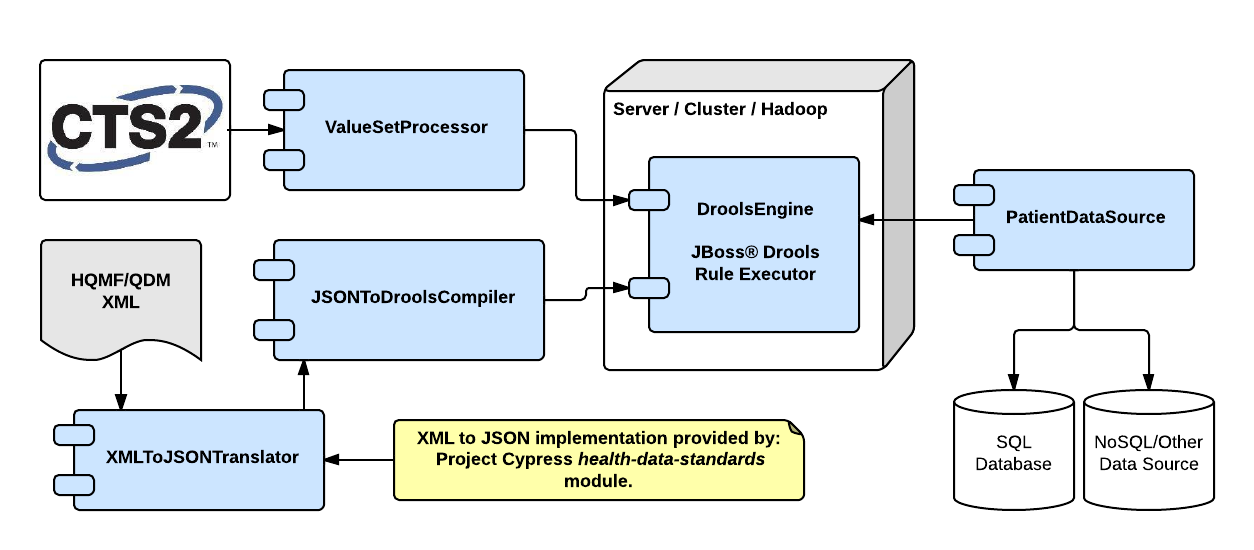
\includegraphics[width=\textwidth]{overall-arch}
\caption{Scalable and High-Throughput Phenotyping Architecture for Clinical Quality Measure Calculation} 
\label{fig:overall_arch}
\end{figure}

\textbf{HQMF/QDM XML to JSON Transformer.}
The HQMF/QDM XML to JSON transformation component parses the HQMF/QDM XML representation and transforms it into easily parsable JSON. This functionality is exposed via a REST service wrapping the Project Cypress health-data-standards\footnote{https://github.com/projectcypress/health-data-standards} project. This component is Ruby\footnote{https://www.ruby-lang.org/en/} based, and represents the only non-Java Virtual Machine (JVM) component of the architecture.

\textbf{JSON to JBoss\textsuperscript{\textregistered} Drools Compiler.}
The QDM JSON representation is then programmatically transformed into executable JBoss\textsuperscript{\textregistered} Drools Rules via a compilation process. The result of this transformation is a single Drools Rule file per measure that is executable by the \textit{Drools Execution Engine} or other JBoss\textsuperscript{\textregistered} Drools environment. The compilation component is based on the Groovy\footnote{http://groovy.codehaus.org/} language, as Groovy provides templating and string interpolation functionality that is difficult to replicate in Java.

\textbf{Drools Execution Engine.}
Utilizing the JBoss\textsuperscript{\textregistered} Drools Rule engine, the generated Drools Rules are executed given an input patient set. The result of this execution is the classification of patients into populations (such as NUMER, DENOM, etc). A thin interface fa\c{c}ade was created over the ``JBoss\textsuperscript{\textregistered} Drools version 5.6.0.Final" library, hiding the implementation details of the engine. There are, in fact, no Drools-related interfaces exposed to the client -- meaning the Drools-based implementation is decoupled from the user-facing contracts.% This was done to allow flexibility in implementation, especially looking forward to a Drools 6.x based implementation and beyond.

\textbf{Patient Data Source.}
Data is provided to the execution engine via an abstraction layer utilizing the Iterator pattern\cite{gamma1993design}. This approach neither provides nor specifies a specific data source, but facilitates custom data extraction implementations tailored to the specific database and environment.

\textbf{Value Set Processor.}
QDM Data Elements semantically define their intended criteria using \textit{Value Sets}, or enumerated sets of coded concepts from standard vocabularies. Take, for instance, the criteria:
\textit{``Diagnosis, Active: Acute Pharyngitis'' using ``Acute Pharyngitis Grouping Value Set (2.16.840.1.113883.3.464.1003.102.12.1011).''}
In this example, in order for the QDM Data Element to be satisfied, a patient record must contain a Diagnosis entry coded with concepts contained in the Value Set uniquely identified by the given HL7 Object Identifier (OID)\cite{steindel2010oids}.

To facilitate this, a mechanism for resolving the concepts of a Value Set is required. This functionality is described in two procedures shown in Algorithm~\ref{alg:value_set_processor}, and defines the capability of the \textit{Value Set Processor}. The procedure \texttt{EXISTS\_IN\_VALUESET} defers explicit full resolution in favor of an \textit{exists}-type functionality, which tests membership of a given $coded\_entry$ within a Value Set. In this procedure, the set of concepts $C$ denotes each concept $c$ defined by the Value Set identified by the given OID. The boolean existence of $coded\_entry$ in $C$ is returned. Furthermore, it often is necessary to find the subset of coded entries that align semantically with a defined Value Set. In the procedure \texttt{FIND\_MATCHES}, instead of checking existence in $C$ as above, the intersection of $C$ and the $coded\_elements$ set is returned. In both procedures, the function $resolve(oid)$ returns the set of all concepts in a Value Set given an OID. 

\begin{algorithm}[H]
\caption{Value Set Processor Functionality}
\label{alg:value_set_processor}
\begin{algorithmic}[1]
\Procedure{exists\_in\_valueset}{oid, coded\_entry}
  \State $C \gets \{c | c \in resolve(oid)\}$
  \State \Return{ $coded\_entry \in C$ }
\EndProcedure
\Procedure{find\_matches}{oid, coded\_elements}
  \State $C \gets \{c | c \in resolve(oid)\}$
  \State \Return{ $C \cap coded\_elements$ }
\EndProcedure
\end{algorithmic}
\end{algorithm}
  
%CTS2 is the recommended implementation of the \textit{Value Set Processor}, and is incorporated via a provided adapter.

\subsection{Processing Algorithms and System Deployment}
\textbf{MapReduce.}
MapReduce is a computational abstraction designed to allow for easier parallelization and distribution of large datasets for processing\cite{dean2008mapreduce}. The computation is a two-step process, consisting of a \textit{map} function followed by a \textit{reduce} function. The \textit{map} function, given an input, divides this input into smaller sub-problems which then are consolidated by the \textit{reduce} function. 

We can apply this concept in the context of patients and populations. In the \textit{map} function, each patient is classified into the appropriate populations given an eCQM. We then \textit{reduce} each population (and its given set of patients) into some analytic result -- for instance, analyzing demographic characteristics or creating patient lists for the quality measure.

\begin{algorithm}[H]
\caption{MapReduce for Clinical Quality Measures}
\label{alg:map_reduce_htp}
\begin{algorithmic}[1]
\State \textbf{map(String measure, List patients)}
%\State \hspace{\algorithmicindent} // key: phenotyping algorithm
%\State \hspace{\algorithmicindent} // values: List of patients
\State \hspace{\algorithmicindent} for each patient in patients:
\State \hspace{\algorithmicindent} \hspace{\algorithmicindent} for each population in \textbf{getPopulations(measure, patient)}:
\State \hspace{\algorithmicindent} \hspace{\algorithmicindent} \hspace{\algorithmicindent} emit(population, patient)
\State \textbf{reduce(String population, Iterator patients)}
%\State \hspace{\algorithmicindent} // key: a population (e.g. IPP, DENOM, etc.)
%\State \hspace{\algorithmicindent} // values: List of patients
\State \hspace{\algorithmicindent} emit(\textbf{postprocess(population, patients)})
\end{algorithmic}
\end{algorithm}

Algorithm~\ref{alg:map_reduce_htp} illustrates the general flow of information through the measure execution logic. The \textit{getPopulations} function encompasses the actual measure execution logic -- in our case, the \textit{Drools Execution Engine} component. The \textit{postprocess} function in the \textit{reduce} portion is left to be implemented by the client, as this will be use case dependent. Note that the current code base includes a basic demographics analytics post processor, but it is expected that clients will extend it to meet their needs, or substitute their own processing entirely.

%\textbf{Clustering.}
%One possible deployment model is to deploy multiple execution nodes in a cluster, currently implemented using a \textit{Master - Worker} computational grid system. With this model, a single \textit{Master} node is responsible for distributing work to several \textit{Worker} nodes. The current implementation follows the Hadoop clustering registration model\cite{wang2009hadoop}, in which worker nodes send a registration request with their network address to the master node. This callback address allows the master node to contact them with task requests. The main advantage of this approach is that the master node does not need a priori knowledge of the number or location of the worker nodes. Clustering could also be implemented using Hadoop itself, utilizing the MapReduce algorithm described.

\subsection{Measure Execution using the JBoss{\textsuperscript{\textregistered}} Drools Rules Engine.}
The JBoss{\textsuperscript{\textregistered}} Drools Rule Engine provides the execution framework for the clinical quality measures. Given the input HQMF/QDM XML, the intermediary JSON representation is then compiled into Drools Rules. Figure~\ref{fig:text_to_drools} shows a representation of CMS MeasureID CMS163v1 and the translation of one example criteria to a Drools Rule. In a Drools Rule execution, decisions are made based on data elements, or \textit{Facts}, that have been placed into working memory either from an external data source or as the result of other rule executions. In this example, a \texttt{MeasurementPeriod} is first checked -- this is a parameter that controls the valid start/end date range of the measure. A \texttt{Patient} is then retrieved from the working memory, and the \texttt{Encounters} of that patient are examined for a \textit{semantic} match (a match in Value Set 2.16.840.1.113883.3.464.1003.101.12.1001), and a \textit{temporal} match (expressed by the \texttt{during} operator in reference to the \texttt{MeasurementPeriod}). Finally, if this result is satisfied, a \texttt{PreconditionResult} is inserted into working memory. The Drools execution engine, using the Rete\cite{forgy1982rete} algorithm, assures that dependent rules will then fire, as the new \texttt{PreconditionResult} is now available in working memory.

\begin{figure}%[H]
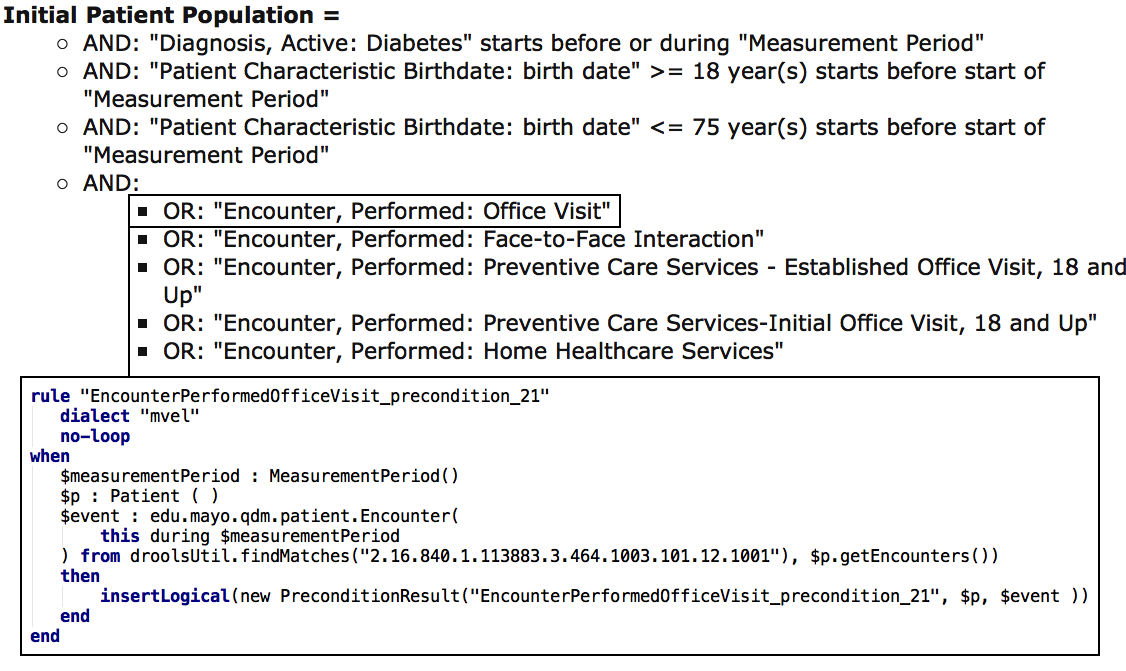
\includegraphics[width=\linewidth]{drools-amia}
\caption{Drools Rule Representation of Initial Patient Population for CMS MeasureID CMS163v1} 
\label{fig:text_to_drools}
\end{figure}

\subsection{Quantitative Evaluation Methods}
\textbf{Performance (Execution Time).}
Scalability and performance are important aspects of the architecture, and the ability to efficiently process large patient sets is critical. Examining the architecture for these aspects requires several components - first, a large de-identified patient set (\textgreater1,000,000 patients with EHR data) is needed. Next, a mechanism to verify the execution results is required to ensure a valid test environment. Finally, as shown in our prior work\cite{thompson2012evaluation}, computational complexity is variable across different quality measures, with examples ranging from simple logical comparisons, to large nested decision trees with temporal relationships between events. We must account for this variability by measuring complexity of the measures under study.

To meet these requirements, the previously mentioned Project Cypress test dataset was re-purposed for execution time performance testing. In order to simulate \textgreater1,000,000 patients, the Project Cypress' 36 patients were ``cloned'' and re-created to form a larger cohort. Execution time was then measured for 12 different patient set sizes, each set size equaling the Project Cypress test patient set size multiplied by an increasing multiple of 2500. Specifically, given the Project Cypress test patient set $P$, we can define each test patient multiset $T_j$ as $T_j = P \otimes (2500j)$ where $1 <= j <= 12$. For each set of test patient data $T_j$, the execution time necessary to compute the test set was measured and recorded.

The complexity of eCQMs under study is an important criteria to quantify, especially when comparing execution times. Several efforts provide guidance in this area\cite{li2012modeling,ross2010analysis}, from which we derive our complexity attributes: \textit{Max Depth,  Boolean Operators, Negations,} and \textit{Temporal Operators}. \textit{Max Depth} measures the maximum amount of nesting in the boolean clauses. If thought of as a boolean decision tree, this measurement would equal the longest path length to the root node. \textit{Boolean Operators} is a count of every \texttt{AND}/\texttt{OR} operator in the measure, while \textit{Negations} measures how many of these operators include a negation. Finally, \textit{Temporal Operators} counts the number of temporal logic calculations specified in the measure -- either as relative temporal comparisons between events, or comparisons to the start and/or end time of the measurement period.

Due to brevity, a subset of the complexity measurements is shown in Table~\ref{fig:qdm_complexity} (See full details at: \url{http://docs.phenotypeportal.org/figures/htp_complexity.png}). To test the computation time of the execution engine under a variety of complexity scenarios, 9 measures representing different complexities were executed. The chosen measures represent a broad spectrum of complexity, ranging from the most complex to relatively straightforward. Execution tests were performed on an Amazon 2xlarge EC2 instance with 8 vCPUs and 30 GiB RAM.

\pgfplotstableset{
begin table=\begin{longtable},
end table=\end{longtable},
}

\begin{table}[H]
\pgfplotstabletypeset[col sep=comma,
header=true,    
columns={CMS ID,Max Depth,Boolean Operators,Negations,Temporal Operators},      
% display specified columns
columns/CMS ID/.style={column type=l,string type},
columns/Max Depth/.style={column type=l,string type},
columns/Boolean Operators/.style={column type=l,string type},
columns/Negations/.style={column type=l,string type},
columns/Temporal Operators/.style={column type=l,string type},
% requires booktabs to place horiz rules
every head row/.style={before row=
\caption{CMS Clinical Quality Measure Algorithm Complexity Metrics}
\label{fig:qdm_complexity}\\\toprule, after row=\midrule\endhead}, 
every last row/.style={after row=\bottomrule}
]{data/complexity/complexity-abbreviated.dat}
\end{table}

\textbf{Performance (Verification).}
Automating the verification of the measure is in many ways as important as the automation of the execution itself. Quality Attribute 2 describes the need for a robust testing environment, and the ability to measure verification performance is key to our architectural evaluation.
Verification was performed using the Project Cypress verification framework, following guidance from the \textit{Test Procedure for \S170.314\copyright\ Clinical Quality Measures} document\cite{project_cypress_test_procedures}. Project Cypress was used as the testing oracle for the verification process, providing a curated test dataset along with expected outcomes. Automation of this verification process also allowed for Test Driven Development\cite{janzen2005test} practices to be used.
To automate this verification process, first the Project Cypress JSON Patient Data was transformed into the target HTP data representation format. Next, the HQMF/QDM XML representation of a given eCQM was selected, and execution of that measure against the test dataset was started. When complete, the results were compared against the expected outcomes, which were loaded from a provided Project Cypress results file.% The output was then recorded and the process repeated until all measures had been tested. Finally, all results were consolidated and analyzed.

\section{\textsc{Results}}

\textbf{Performance (Execution Time).}
Execution times, shown in Figure~\ref{fig:execution_time}, show the total elapsed execution time over the test patient sets. Execution times tended to scale linearly as the patient set size increased. The execution time of CMS MeasureID CMS145v1 \textit{Beta-Blocker Therapy—Prior Myocardial Infarction (MI) or Left Ventricular Systolic Dysfunction (LVEF $<40\%$)} was anomalous, as shown in the results. Although similar in measured complexity compared to other executed measures, it exhibited a significantly higher execution time.

\begin{figure}[H]
\centering
\begin{tikzpicture}
\begin{axis}[
    xlabel={Patients},ylabel={Elapsed Time (seconds)}, 
    width=\linewidth, height=7.5cm,
    xmin=0,
    xmax=1000000,
    ymin=0,
    grid=major,
    xticklabel style={
            /pgf/number format/fixed
    },
    scaled x ticks=false,
    legend pos= north west]

\addlegendimage{empty legend}
\addlegendentry{\textbf{CMS MeasureID}}
\addplot[color=blue,mark=pentagon*] table[x index=0,y index=1,col sep=comma] {data/execution/0036.dat};
\addlegendentry{CMS126v1}
\addplot[color=red,mark=square*] table[x index=0,y index=1,col sep=comma] {data/execution/0043.dat};
\addlegendentry{CMS127v1}
\addplot[color=green,mark=diamond*] table[x index=0,y index=1,col sep=comma] {data/execution/0062.dat};
\addlegendentry{CMS134v1}
\addplot[color=black,mark=diamond*,dashed] table[x index=0,y index=1,col sep=comma] {data/execution/0070.dat};
\addlegendentry{CMS145v1}
\addplot[color=black,mark=x] table[x index=0,y index=1,col sep=comma] {data/execution/0060.dat};
\addlegendentry{CMS148v1}
\addplot[color=olive,mark=triangle*,dashed] table[x index=0,y index=1,col sep=comma] {data/execution/0033.dat};
\addlegendentry{CMS153v1}
\addplot[color=green,mark=pentagon*,dashed] table[x index=0,y index=1,col sep=comma] {data/execution/0710.dat};
\addlegendentry{CMS159v1}
\addplot[color=blue,mark=square*,dashed] table[x index=0,y index=1,col sep=comma] {data/execution/0712.dat};
\addlegendentry{CMS160v1}
\addplot[color=black,mark=*] table[x index=0,y index=1,col sep=comma] {data/execution/0064.dat};
\addlegendentry{CMS163v1}

\end{axis}
\end{tikzpicture}
\caption{CMS Clinical Quality Measure Algorithm Execution Time} 
\label{fig:execution_time}
\end{figure}

\textbf{Performance (Verification).}
A subset of the Project Cypress validation results are shown in Table~\ref{fig:qdm_verification}. For each measure, results are displayed in the form of \textit{(actual/expected)} patients classified for the given population. Of the 58 total measures analyzed, 56 matched the expected results, while 2 measures failed to match the expected results in one or more of the population criteria. The two anomalous measures, CMS MeasureIDs CMS159v1 and CMS122v1, both failed to correctly identify the \textit{Numerator} (NUMER) population. Due to brevity, see detailed results here: \url{http://docs.phenotypeportal.org/figures/htp_cypress.png}.

\pgfplotstableset{
    row style/.style 2 args={
        postproc cell content/.append code={%
            \count0=\pgfplotstablerow
            \advance\count0 by1\relax
            \ifnum\count0=#1
                \pgfkeysalso{#2}%
            \fi
        }
    }
}

\begin{table}%[H]
\pgfplotstabletypeset[col sep=comma,
header=true,    
row style={1}{@cell content=\bfseries #1},
row style={8}{@cell content=\bfseries #1},
columns={CMS ID,IPP,NUMER,DENOM,DENEX,DENEXCEP,Result},
% display specified columns
columns/CMS ID/.style={column type=l,string type},
columns/IPP/.style={column type=l,string type},
columns/NUMER/.style={column type=l,string type},
columns/DENOM/.style={column type=l,string type},
columns/DENEX/.style={column type=l,string type},
columns/DENEXCEP/.style={column type=l,string type},
columns/Result/.style={column type=l,string type},
% requires booktabs to place horiz rules
every head row/.style={before row=
\caption{Project Cypress Verification Results - Patients Classified per Population \textit{(actual/expected)}
\label{fig:qdm_verification}}\\\toprule, after row=\midrule\endhead}, 
every last row/.style={after row=\bottomrule}
]{data/verification/cypress_verification-abbreviated.dat}
\end{table}

\section{\textsc{Discussion}}
\textbf{Summary.}
The evaluation of the candidate architecture begins with ensuring that the Architectural Quality Attributes still hold. By using standards such as QDM/HQMF and CTS2, along with the uniform interface of REST, we were able to achieve a degree of \textit{Interoperability} in the system. Also, as shown by the Project Cypress integration, the architecture was able to achieve a high degree of \textit{Testability}, while the MapReduce processing algorithm enables a solid platform for high system \textit{Scalability}.
Our quantitative analysis results also verify that the Quality Attributes hold. Achieving 96.4\% Cypress verification (56 out of 58 measures) shows high system ``correctness,'' while the execution time results show predictable and scalable results for the selected measures given datasets of \textgreater1,000,000 patients. 

\textbf{Anomalous Results.}
CMS MeasureIDs CMS159v1 and CMS122v1 both failed to produce the correct results when executed against Project Cypress test data. For CMS159v1, the numerator population is defined by
\textit{``Risk Category Assessment: PHQ-9 Tool (result $<$ 5 )'' $<=$ 13 month(s) starts after end of ``Occurrence A of Risk Category Assessment: PHQ-9 Tool.''}
Cypress verification results identify test patient \texttt{BH\_Adult\_D} for inclusion, and test data for this patient shows two qualifying assessments, the first on \textit{Sat, 24 Sep 2011 12:30:00 GMT} and the second on \textit{Thu, 01 Nov 2012 12:30:00 GMT}. Our results exclude this patient via the $<=$ 13 month(s) temporal constraint. It is unclear as to whether this is a misinterpretation of the temporal constraint or an otherwise unknown system defect.

With regard to the verification failure of CMS122v1, the test patient \texttt{Diabetes\_Adult\_A} was erroneously added to the numerator population due to a miscalculation of the the constraint:
\textit{``Occurrence A of Laboratory Test, Result: HbA1c Laboratory Test (result $>$ 9 \%).''} This patient does have an HbA1c Laboratory Test result, but with a value of only 8\%. Inclusion of this test patient indicates a system defect in analyzing the value of this laboratory test result.

The anomalous execution time of CMS145v1 is not sufficiently explained by complexity calculations in Table~\ref{fig:qdm_complexity}, as it does not differ significantly from other observed measures. One possible explanation could be the large number of individual Drools Rules produced by the compilation process of this measure. To explore this further, Figure~\ref{fig:qdm_drools_rules_generation} shows the number of generated Drools Rules as compared to execution time for each analyzed measure. The results indicate a possible correlation between the two, and shows the execution time of CMS145v1 degrades predictably given the large number of discrete Drools Rules needed to express it.

\begin{figure}%[H]
\centering
\begin{tikzpicture}
\begin{axis}[
    xlabel={Generated Drools Rules},ylabel={Elapsed Time (seconds)}, 
    width=\linewidth, height=6cm,
    xmin=0,
    xmax=1200,
    ymin=0,
    grid=major,
    xticklabel style={
            /pgf/number format/fixed
    },
    scaled x ticks=false,
    legend pos= south east]
     \node [below] at (axis cs:  1111,  575) {CMS145v1};
     \addplot[smooth,dashed] plot coordinates {
                    (0,50)
                    (1200,700)
                };

    \addplot[only marks] table[x index = 0, y index= 1,col sep=comma] {data/rules/scatter.dat};

\end{axis}
\end{tikzpicture}
\caption{Measure Execution Time per 1,000,000 Patients vs. Number of Generated Drools Rules} 
\label{fig:qdm_drools_rules_generation}
\end{figure}

\textbf{Limitations.}
Compilation of the QDM XML into JBoss\textsuperscript{\textregistered} Drools Rules has several significant opportunities for improvement. First, Drools Fusion and Complex Event Processing\cite{bali2013drools} was only partially utilized for the temporal relationships. Utilizing these modules would cause a significant increase in rule readability and conciseness. Next, the generated rules are prone to combinatorial explosions of rule activations -- especially in measures that heavily utilize \texttt{OR} clauses. The \texttt{exists} Drools operator would usually alleviate this, but a unique aspect of the QDM measures called \textit{Specific Occurrences} makes this difficult. A \textit{Specific Occurrence} is the notion of assigning an identifier to a specific event (such as a Diagnosis or Encounter), and referring to that specific event elsewhere in the measure. To account for this, we follow the \textit{Specific Occurrence} processing algorithm proposed by the MITRE Corporation\cite{specific_occurences}.
Execution time performance metrics are also limited by the small Project Cypress patient set size, and as such, a larger test patient set would be more appropriate for scalability and performance evaluations.

\textbf{Future Work.}
In general, optimizing the Drools Rule compilation has the potential to increase scalability and performance to even higher levels, as well as to provide more readable and concise rules.
Also, the relationship between Complexity in Table~\ref{fig:qdm_complexity} and Execution Time in Figure~\ref{fig:execution_time} is not fully understood. If a correlation exists, it has not been statistically analyzed. Furthermore, asserting relative complexity rankings between measures is error-prone, as algorithms and metrics for capturing true measure ``complexity'' are not known. More analysis is needed to explore how this complexity can be measured. Along these lines, Figure~\ref{fig:qdm_drools_rules_generation} suggests that the number of generated Drools Rules -- not complexity -- may be a more accurate model of execution time. If the correlation does indeed hold, future work in Drools Rule compilation optimizations may be approached with that model in mind.

\textbf{Acknowledgement.} This work has been supported in part by funding from the National Institutes of Health (R01-GM105688).

% unstr is used to keep citation order
\bibliographystyle{unsrt}
\setlength{\bibsep}{0.0pt}
\bibliography{htp-amia}

\end{document}
